\documentclass[a4paper,11pt,article]{memoir}

\usepackage[utf8]{inputenc}
\usepackage{fourier}
\usepackage{amsmath,amssymb}
\usepackage{xstring,ifthen,xcolor}
\usepackage{xspace}

\usepackage{tikz}
\usepackage{pgfmath}
\usetikzlibrary{calc,shapes,positioning}

\title{Mini-Mapper 8:\,Photoencoder signals}
\author{Ian~Ross}

\newdimen\holecircleradius{}
\pgfmathsetlength{\holecircleradius}{10mm}

\newdimen\offsetangle{}

\newcommand{\fulldisk}[1]{%
\pgfmathsetlength{\offsetangle}{#1}
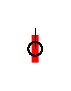
\begin{tikzpicture}[scale=1.75]
  \fill[fill=red]
  (-0.25mm,\the\holecircleradius-1mm) --
  (-0.25mm,\the\holecircleradius+1mm) --
  (0.25mm,\the\holecircleradius+1mm) --
  (0.25mm,\the\holecircleradius-1mm) --
  (-0.25mm,\the\holecircleradius-1mm);

  \draw (0,0) -- (0,\the\holecircleradius+1.5mm);
  \draw (0,0) -- (90+\the\offsetangle:\the\holecircleradius+1.5mm);

  \draw[dashed] (0,0) circle [radius=\the\holecircleradius];

  \foreach \angle in {0,1,...,31}
    \draw (360/32*\angle+90+\the\offsetangle:\the\holecircleradius) circle [radius=0.5mm];
\end{tikzpicture}}

\graphicspath{{figs/}}

\begin{document}

\maketitle

\section*{Introduction}

The idea here is to calculate the form of signal that the
phototransistor in the photointerrupter on the motor encoder disk will
generate as the encoder disk rotates. This isn't strictly necessary,
but it's mildly interesting, and a fun geometrical exercise.
Figure~\ref{fig:setup} shows the basic setup, with the ring of holes
in the encoder disk rotating past the beam of the photointerrupter.

The important factor for the purposes of determining the current
signal generated by the phototransistor in the photointerrupter is the
area of overlap between the hole in the encoder disk and the beam of
infrared radiation emitted by the photodiode in the photointerrupter.

The following parameters are used in the analysis below:
\begin{itemize}
  \item{$d$: the diameter of a single hole in the encoder disk;}
  \item{$D$: the diameter of the circle of centres of the holes in the
    encoder disk;}
  \item{$w$ and $h$: the width and height of the beam from the
    photodiode in the photointerrupter --- for the photointerrupters
    I've been looking at, the beam aperture is rectangular, with the
    narrower dimension horizontal.}
  \item{$\phi$: the angle (anticlockwise positive) between the line
    between the centre of rotation of the encoder disk and the center
    of the photointerrupter beam, and the line betwen the centre of
    rotation of the encoder disk and the centre of the hole under
    consideration.}
\end{itemize}

We make a few assumptions:
\begin{enumerate}
  \item{$d \leq h$ and $d \geq w$: these assumptions give the
    geometrical relations between the optical beam and the hole as
    shown in Figure~\ref{fig:setup}, i.e., the outline of the hole has
    either zero, two or four intersections with the outline of the
    optical beam, with all intersections occurring on the vertical
    sides of the beam.}
  \item{The gaps between the holes in the encoder disk are large
    enough that only one hole can intersect with the optical beam at a
    time.}
\end{enumerate}

\begin{figure}
  \begin{center}
    \fulldisk{0}\hspace{0.5cm}\fulldisk{1}\hspace{0.5cm}\fulldisk{2}
  \end{center}

  \begin{center}
    \fulldisk{3}\hspace{0.5cm}\fulldisk{4}\hspace{0.5cm}\fulldisk{5}
  \end{center}

  \caption{Photointerrupter beam (red, $w = 0.5\,\mathrm{mm} \times h
    = 2\,\mathrm{mm}$) interfacing with holes in motor encoder disk.
    Dashed circle shows line of centres of encoder disk holes
    (diameter $D = 20\,\mathrm{mm}$), with each hole being of diameter
    $d = 1\,\mathrm{mm}$. The images here show the positions of the
    encoder disk $1^\circ$ apart, starting with a hole centrally
    located in front of the photointerrupter beam ($\phi = 0$) and
    showing positions of $\phi = 1^\circ, 2^\circ, 3^\circ, 4^\circ,
    5^\circ$.}\label{fig:setup}
\end{figure}

\section*{Intersections of holes with optical aperture}

Let's think about the overlap of a single hole with the aperture of
the photointerrupter. We'll consider only $\phi \geq 0$ (the situation
for negative $\phi$ is symmetrical). Writing $R = D / 2$ for the
radius of the circle of centres, and $r = d / 2$ for the radius of the
holes, the centre of the hole we're looking at is at $(x_c, y_c)$:
\begin{equation*}
  x_c = -R \sin \phi, \; y_c = R \cos \phi
\end{equation*}
and its equation is
\begin{equation*}
  {(x - x_c)}^2 + {(y - y_c)}^2 = r^2
\end{equation*}
or
\begin{equation*}
  {(x + R \sin \phi)}^2 + {(y - R \cos \phi)}^2 = r^2
\end{equation*}
Points of intersection of this circle with the outline of the optical
beam are given by solving this equation for $y$ when $x = \pm w/2$:
\begin{equation*}
  R^2 \sin^2 \phi \pm w R \sin \phi + w^2/4 + y^2 - 2 R y \cos \phi +
  R^2 \cos^2 \phi - r^2 = 0
\end{equation*}
or, simplifying
\begin{equation}
  \label{eq:intersection}
  y^2 - 2 R y \cos \phi + R^2 - r^2 + w^2/4 \pm w R \sin \phi = 0.
\end{equation}
This discriminant of this equation is
\begin{equation}
  \label{eq:discriminant}
  \Delta_{\pm} = 4 R^2 \cos^2 \phi \mp 4 w R \sin \phi - 4 (R^2 - r^2)
  - w^2.
\end{equation}
Figure~\ref{fig:discriminant} shows values of $\Delta_{\pm}$
from~\eqref{eq:discriminant} as a function of $\phi$. When the hole
extends right across the width of the optical beam aperture, there are
four intersections between the circle defining the outline of the hole
and the outline of the aperture. In this case, $\Delta_{+} \geq 0,
\Delta_{-} \geq 0$. When the outline of the hole intersects with only
one vertical side of the optical beam aperture, then there are two
intersections between the circle and the outline of the aperture and
$\Delta_{+} < 0, \Delta_{-} \geq 0$. When there are no intersections
between the circle and the outline of the aperture then both
discriminants are negative.

The limits in terms of the angular displacement $\phi$ of the ranges
with solutions are given by $\Delta_{\pm} = 0$.
From~\eqref{eq:discriminant}, this gives
\begin{equation*}
  4 R^2 \sin^2 \phi \pm 4 w R \sin \phi - 4 r^2 + w^2 = 0
\end{equation*}
or
\begin{align*}
  \sin \phi &= \frac{\mp 4 w R \pm \sqrt{16 w^2 R^2 - 16 R^2 (w^2 - 4 r^2)}}{8 R^2} \\
  \sin \phi &= \frac{\mp w \pm \sqrt{w^2 - (w^2 - 4 r^2)}}{2 R} \\
  \sin \phi &= \frac{\mp w \pm 2 r}{2 R}
\end{align*}

\begin{equation*}
  \sin \phi = \frac{\mp w/2 \pm r}{R}.
\end{equation*}
The four limiting values for $\phi$ derived from this equation provide
the limits of the two intersection and four intersection cases in the
positive and negative $\phi$ directions. Putting $w =
0.5\,\mathrm{mm}$, $r = 0.5\,\mathrm{mm}$ and $R = 10\,\mathrm{mm}$,
we get limits of $|\phi| \leq 4.30^\circ$ for the two intersections
case, and $|\phi| \leq 1.43^\circ$ for the four intersections case,
which matches with the limits seen in Figure~\ref{fig:discriminant}.

\begin{figure}
  \begin{center}
    \includegraphics[width=\textwidth]{intersection-discriminant}
  \end{center}

  \caption{Discriminant for hole/beam intersection equation as a
    function of angular displacement $\phi$. The boundary of the ``two
    intersections'' region is $\Delta_{-}(\phi)$, while that of the
    ``four intersections'' region is $\Delta_{+}(\phi)$.}\label{fig:discriminant}
\end{figure}

Solutions to the positive and negative versions
of~\eqref{eq:intersection} exist when $\Delta_{\pm} \geq 0$ and are
given by:
\begin{equation}
  \label{eq:solutions}
  y_{\color{black}\pm}^{\color{red}\pm} = R \cos \phi {\color{red}\pm} \frac12
  \sqrt{\Delta_{\pm}} = y_c {\color{red}\pm} \frac12
  \sqrt{\Delta_{\pm}}
\end{equation}
(The sign of the discriminant $\Delta_{\pm}$ matches the sign on the
left hand side. The other plus-or-minus sign is for the usual pair of
solutions to a quadratic equation, and corresponds to the two members
of the pairs of intersection points.) Figure~\ref{fig:solutions} shows
these solutions as a function of $\phi$.

\begin{figure}
  \begin{center}
    \includegraphics[width=\textwidth]{intersection-solutions}
  \end{center}

  \caption{Solutions for hole/beam intersection equation as a function
    of angular displacement $\phi$. The $y_{-}$ values show
    intersections with the left-hand edge of the optical aperture
    (remember positive $\phi$ means movement of the hole to the left
    from top dead centre), and $y_{+}$ values are for intersection
    with the right-hand edge of the aperture. The ``(pos)'' and
    ``(neg)'' labels indicate the two signs in~\eqref{eq:solutions}
    for the two solutions to each quadratic
    equation.}\label{fig:solutions}
\end{figure}

\section*{Hole/aperture overlap area}

Given the intersection information from~\eqref{eq:solutions}, we now
need to calculate the area of the overlap between the encoder disk
hole and the photointerrupter optical aperture. There are three cases
to consider, two requiring calculation and one trivial:
\begin{enumerate}
  \item{There are two intersections between the outline of the hole
    and the optical aperture. In this case, the overlap between the
    hole and aperture is formed by a line segment of the vertical side
    of the aperture and a segment of the circle forming the outline of
    the hole --- this segment lies inside the optical aperture and has
    endpoints given by the intersection points between the hole and
    the vertical side of the aperture (Figure~\ref{fig:overlaps}a).}
  \item{There are four intersections between the outline of the hole
    and the optical aperture. In this case, the overlap is the encoder
    disk hole minus two segments of the circle forming the outline of
    the hole --- these segments lie outside the optical aperture and
    have endpoints given by the intersection points between the hole
    and the vertical sides of the aperture
    (Figure~\ref{fig:overlaps}b).}
  \item{There are no intersections between the outline of the encoder
    disk hole and the optical aperture. In this trivial case, the
    overlap area is identically zero.}
\end{enumerate}
In each of the two cases requiring calculation, the calculation can be
performed on the basis of an expression for the area of a segment of a
circle. For a circle with radius $R$, the area $A$ of a segment
subtending an angle $\theta$ at the centre of the circle is
\begin{equation}
  \label{eq:segment}
  A = \frac{R^2}{2} (\theta - \sin \theta).
\end{equation}

\begin{figure}
  \begin{center}
    \begin{tabular}{cc}
    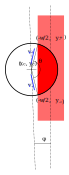
\includegraphics[height=0.6\textheight]{overlap-2} &
    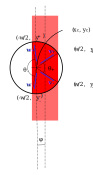
\includegraphics[height=0.6\textheight]{overlap-4} \\
    (a) Two intersections & (b) Four intersections
    \end{tabular}
  \end{center}

  \caption{Overlap cases: (a) two intersections, so overlap is a
    segment of a circle; (b) four intersections, so overlap is a
    circle minus two segments.}\label{fig:overlaps}
\end{figure}

\subsection*{Case 1: two intersections}

Figure~\ref{fig:overlaps}a shows this case. The intersection points of
the outline of the encoder disk hole and the optical aperture are
$(-w/2, y_{-}^{+})$ and $(-w/2, y_{-}^{-})$. We know the radius of the
encoder disk hole, so in order to apply~\eqref{eq:segment} to
calculate the area of overlap, we need to find the angle $\theta$. To
do this, we construct vectors $\mathbf{v}_{+}$ and $\mathbf{v}_{-}$
between the centre of the encoder disk hole and the intersection
points:
\begin{equation}
  \mathbf{v}_{+} = \begin{pmatrix}
    -w/2 - x_c \\
    y_{-}^{+} - y_c
  \end{pmatrix}, \;\;\;\;\;\;
  \mathbf{v}_{-} = \begin{pmatrix}
    -w/2 - x_c \\
    y_{-}^{-} - y_c
  \end{pmatrix},
\end{equation}
and then
\begin{equation*}
  \cos \theta = \hat{\mathbf{v}}_{+} \cdot \hat{\mathbf{v}}_{-}.
\end{equation*}
(Here $\hat{\mathbf{v}}$ is the unit vector in the direction of vector
$\mathbf{v}$.) First we calculate $\mathbf{v}_{+} \cdot
\mathbf{v}_{-}$, making use of the fact that $y_{-}^{\pm} - y_c = \pm
\frac12 \sqrt{\Delta_{-}}$ (from~\eqref{eq:solutions}):
\begin{equation}
  \mathbf{v}_{+} \cdot \mathbf{v}_{-} = {\left(\frac{w}{2} +
    x_c\right)}^2 + (y_{-}^{+} - y_c) (y_{-}^{-} - y_c) =
         {\left(\frac{w}{2} + x_c\right)}^2 - \frac{\Delta_{-}}{4}.
\end{equation}
Now, we also find that
\begin{align*}
  |\mathbf{v}_{\pm}|^2 = {\left(\frac{w}{2} + x_c\right)}^2 + {(y_{-}^{\pm} -
  y_c)}^2 = {\left(\frac{w}{2} + x_c\right)}^2 + \frac{\Delta_{-}}{4}.
\end{align*}
so that
\begin{equation*}
  |\mathbf{v}_{+}| |\mathbf{v}_{+}| = {\left(\frac{w}{2} +
    x_c\right)}^2 + \frac{\Delta_{-}}{4}
\end{equation*}
and we finally arrive at
\begin{equation*}
  \cos \theta = \frac{\mathbf{v}_{+} \cdot
    \mathbf{v}_{-}}{|\mathbf{v}_{+}| |\mathbf{v}_{+}|} =
  \frac{{\left(\frac{w}{2} + x_c\right)}^2 -
    \frac{\Delta_{-}}{4}}{{\left(\frac{w}{2} + x_c\right)}^2 +
    \frac{\Delta_{-}}{4}}
\end{equation*}
which gives an area for the two intersection case of
\begin{equation*}
  A_2 = \frac{r^2}{2} (\theta - \sin \theta)
\end{equation*}

\subsection*{Case 2: four intersections}

The four intersections case (Figure~\ref{fig:overlaps}b) is similar,
except that we have two angles, $\theta_{-}$ and $\theta_{-}$, one of
each side of the optical aperture, and the area of interest is the
total area of the encoder disk hole minus the area of the two segments
subtended by $\theta_{-}$ and $\theta_{-}$.

The left-hand side of Figure~\ref{fig:overlaps}b can be treated the
same way as for the two intersections case:
\begin{equation}
  \cos \theta_{-} = \frac{\mathbf{w}_{+} \cdot
    \mathbf{w}_{-}}{|\mathbf{w}_{+}| |\mathbf{w}_{+}|} =
  \frac{{\left(\frac{w}{2} + x_c\right)}^2 -
    \frac{\Delta_{-}}{4}}{{\left(\frac{w}{2} + x_c\right)}^2 +
    \frac{\Delta_{-}}{4}}.
\end{equation}
The right-hand side goes the same kind of way, with vectors
$\mathbf{v}_{+}$ and $\mathbf{v}_{-}$ defined as:
\begin{equation}
  \mathbf{v}_{+} = \begin{pmatrix}
    w/2 - x_c \\
    y_{+}^{+} - y_c
  \end{pmatrix}, \;\;\;\;\;\;
  \mathbf{v}_{-} = \begin{pmatrix}
    w/2 - x_c \\
    y_{+}^{-} - y_c
  \end{pmatrix},
\end{equation}
so that
\begin{equation}
  \mathbf{v}_{+} \cdot \mathbf{v}_{-} = {\left(\frac{w}{2} -
    x_c\right)}^2 + (y_{+}^{+} - y_c) (y_{+}^{-} - y_c) =
         {\left(\frac{w}{2} - x_c\right)}^2 - \frac{\Delta_{+}}{4}.
\end{equation}
and
\begin{align*}
  |\mathbf{v}_{\pm}|^2 = {\left(\frac{w}{2} - x_c\right)}^2 + {(y_{+}^{\pm} -
  y_c)}^2 = {\left(\frac{w}{2} - x_c\right)}^2 + \frac{\Delta_{+}}{4}.
\end{align*}
so that
\begin{equation*}
  |\mathbf{v}_{+}| |\mathbf{v}_{+}| = {\left(\frac{w}{2} -
    x_c\right)}^2 + \frac{\Delta_{+}}{4}
\end{equation*}
and we arrive at
\begin{equation*}
  \cos \theta_{+} = \frac{\mathbf{v}_{+} \cdot
    \mathbf{v}_{-}}{|\mathbf{v}_{+}| |\mathbf{v}_{+}|} =
  \frac{{\left(\frac{w}{2} - x_c\right)}^2 -
    \frac{\Delta_{+}}{4}}{{\left(\frac{w}{2} - x_c\right)}^2 +
    \frac{\Delta_{+}}{4}}.
\end{equation*}
The total area in the four intersections case is then:
\begin{equation*}
  A_4 = \pi r^2 - \frac{r^2}{2} (\theta_{+} - \sin \theta_{+}) -
  \frac{r^2}{2} (\theta_{-} - \sin \theta_{-}).
\end{equation*}

\section*{Final results}

The functional dependence of the overlap area between an encoder disk
hole and the optical beam of the interrupter is shown in
Figure~\ref{fig:overlap-areas}, representing the overlap as the
fraction of the photointerrupter optical beam covered by the encoder
hole disk. The assumption is that the current generated by the
phototransistor in the photointerrupter will be proportional to this
fractional overlap.

We can now use these results to generate simulated photocurrent
signals for use in simulations.

\begin{figure}
  \begin{center}
    \includegraphics[width=\textwidth]{overlap-areas}
  \end{center}

  \caption{Dependence of fraction of area of photointerrupter optical
    beam covered by encoder disk hole as a function of angular
    displacement $\phi$, based on $w = 0.5\,\mathrm{mm}$, $r =
    0.5\,\mathrm{mm}$ and $R = 10\,\mathrm{mm}$.}\label{fig:overlap-areas}
\end{figure}

\section*{Generation of simulated signals}

Based on the results so far, we want to be able to generate PWL
(piecewise linear) data files for use in LTSpice simulations. We'll do
this with a Python script. Basically, the script just duplicates the
calculations performed above, and produces a time series of simulated
phototransistor current values, based on a time profile of wheel
velocity. We assume that the phototransistor current is proportional
to the fraction of the optical aperture that is overlapped by the
motor encoder disk hole.

The calculations go something like this, stepping the simulation time
by a constant timestep (I've been using $\Delta t = 0.1\,\mathrm{ms}$):
\begin{enumerate}
  \item{Determine the current linear velocity from the current
    simulation time. The example I've been using starts from rest,
    accelerates to a constant speed, has a constant velocity segment,
    then decelerates back to rest. Acceleration and deceleration are
    both eased using a parabolic easing function.}
  \item{Step the current distance, wheel angle and encoder disk angle
    using simple Euler integration.}
  \item{Normalise the encoder disk angle into the range $|\phi| \leq
    \Delta \phi / 2$, where $\Delta \phi$ is the angular separation
    between adjacent holes in the encoder disk.}
  \item{We can then apply the calculations in the first part of this
    document to the angle $\phi$ to get the area overlap fraction
    between the optical aperture and the hole in the encoder disk.}
  \item{Multiply the area overlap fraction by the maximum light
    current generated by the phototransistor (I'm using
    $I_L(\mathrm{max}) = 2\,\mathrm{mA}$, which is based on the
    ``typical'' value for the Vishay TCST1230 photointerrupter I'm
    planning to use.)}
\end{enumerate}
The results of this procedure are shown in
Figure~\ref{fig:simulation}.

\begin{figure}
  \begin{center}
    \includegraphics[width=\textwidth]{simulation-1}
  \end{center}
  \begin{center}
    \includegraphics[width=\textwidth]{simulation-2}
  \end{center}
  \begin{center}
    \includegraphics[width=\textwidth]{simulation-3}
  \end{center}
  \begin{center}
    \includegraphics[width=\textwidth]{simulation-4}
  \end{center}

  \caption{Simulated phototransistor current based on using a Vishay
    TCST1230 photointerrupter, an encoder disk with 32 holes of 1\,mm
    diameter on a 20\,mm diameter circle, and a linear velocity
    profile starting from rest, increasing to 50\,mm/s in 3 seconds,
    travelling at constant speed for 2 seconds, then decelerating back
    to rest in 3 seconds.}\label{fig:simulation}
\end{figure}


\end{document}
